%\documentclass[11pt,twocolumn]{article}
%\usepackage{graphicx}
%\usepackage{fancyhdr}
%\usepackage{amssymb,amsmath}
%\usepackage[usenames,dvipsnames]{color}
%\usepackage[colorlinks,citecolor=RedViolet,urlcolor=blue]{hyperref}
%\usepackage{doi}
%\usepackage{setspace}
%\usepackage[paperwidth=8.5in, paperheight=11in,top=1in, bottom=1in, left=1in, r%ight=1in]{geometry}
%\usepackage[compact]{titlesec}
%\usepackage{abstract}
%\usepackage[position=t,singlelinecheck=off,justification=raggedleft]{subcaption}
%\usepackage[authoryear,square]{natbib}
%\usepackage{aas_macros}
%\usepackage{array}
%\pagestyle{fancy}
%\fancyhead[R]{Veibell \thepage}
%\fancyhead[L]{}

%\newcolumntype{L}{>{$}l<{$}} %To enable math mode in tables (for saying things like B_z)
%\newcolumntype{C}{>{$}c<{$}}
%\newcommand{\vinote}[1]{\textcolor{red}{\textbf{#1}}} %If you want \inote{#} instead of just \note #, for inline notes
%\def\vnote#1\par{\textcolor{red}{\textbf{#1}}\\} %Make note bold and red, re-add newline
%\newcommand{\req}{\ensuremath{\rho_{eq}}}
%\newcommand{\inote}[1]{\textcolor{blue}{\textbf{#1}}} %Inline notes in blue
%\def\note#1\par{\textcolor{blue}{\textbf{#1}}\\} 

\documentclass[12pt]{article}
\bibliographystyle{./style/agufull}
\usepackage[square,comma,authoryear]{natbib}
\usepackage{aas_macros}
\usepackage{epsfig}
\usepackage{amsmath}
\usepackage{style/lineno}
%\usepackage{booktabs}
\linenumbers*[1]
\usepackage{subfig}

\usepackage{setspace}  
\usepackage{fancyhdr}

\newcommand{\citeay}[1]{%
\citeauthor{#1}, \citeyear{#1}%
}

\pagestyle{fancy}
\fancyhead{}
\fancyfoot{}
\fancyhead[R]{X - \thepage}
\fancyhead[L]{VEIBELL: MASS DENSITY AT GEO}
\fancyfoot[L]{D R A F T}
\fancyfoot[C]{\today}
\fancyfoot[R]{D R A F T}
\renewcommand{\headrulewidth}{0.0pt}
\renewcommand{\footrulewidth}{0.0pt}

\oddsidemargin 0.0in
\evensidemargin 1.0in
\textwidth 6.5in
\headheight 0.1in
\topmargin -0.5in
\textheight 9.0in

\begin{document}
\title{Average solar wind and geomagnetic activity influence on the equatorial plasma mass density at geosynchronous orbit}
\author{V. Veibell and R.S. Weigel}
\doublespacing
\maketitle

%\author{
%Victoir Veibell\footnote{vveibell@gmu.edu}
%\and
%R.S. Weigel\footnote{rweigel@gmu.edu}}

%\setlength{\parskip}{3ex}

%\titlespacing{\section}{0pc}{0.2pc}{-1pc}
%\titlespacing{\subsection}{0pc}{0.1pc}{-1pc}
%\titleformat*{\section}{\normalsize\bfseries}
%\titleformat*{\subsection}{\small\bfseries}

%\twocolumn[
%  \begin{@twocolumnfalse}
%\maketitle
%\hrule
\begin{abstract}
We consider two types of events, identified by decreases in $D_{st}$ below a threshold value and increases in the the equatorial mass density at geosynchronous altitudes, $\rho_{eq}$, above a threshold value on 1-hour and 1-day time scales using the \cite{Takahashi2010} dataset.  From the $D_{st}$ events, we find that there is a weak and small amplitude ($< 10$\%) difference between $\rho_{eq}$ on the day of the event and the days before and after on both daily and hourly timescales.  Although very large geomagnetic storms have been observed to correspond to large increases in $\rho_{eq}$, on average, $\rho_{eq}$ following the onset of a geomagnetic storm does not depend on the north-south component of the interplanetary magnetic field, $B_z$ near onset time. From the $\rho_{eq}$ events, we find a weak dependence on $B_{z}$ after the onset of an event, with higher average $B_{z}$ four hours after the event onset corresponding to larger $\rho_{eq}$ events.  In contrast, the average of $B_z$ four hours prior to $\rho_{eq}$ events does not have a statistically significant impact on $\rho_{eq}$ after onset.
\end{abstract}
%\vspace{2em}
%\hrule
%\vspace{2em}
% \end{@twocolumnfalse}
%  ]

%\saythanks

\section{Introduction}

%The plasma trough is a transition region between the higher density and lower temperature plasmasphere and the lower density and higher energy magnetosphere \citep{Mayr1968ModelMagnetosphereTemperature} and is .  Inside of the plasmapause, the density is primarily due to ionospheric photoionization; outside of the plasmapause, the density has contributions from the co-rotating plasmasphere and Earthward convecting magnetosphere plasmas.

The dependence of the plasmapause location on geomagnetic activity was observed as early as \cite{Carpenter1966} and there are well--validated models of the plasmapause location as a function of $L$, $MLT$, and geomagnetic activity (\cite{LemaireEarthsPlasmasphere}, \cite{Moldwin2002ModelPlasmapause}, \cite{OBrien2003EmpiricalPlasmapause}).  Models also exist for the plasmasphere density (\cite{Gallagher1988EmpiricalModelPlasmasphere}; \cite{LemaireEarthsPlasmasphere}) with similar parameterization.

The dependence of the plasma density outside of the nominal plasmapause location on geomagnetic and solar wind conditions has not been extensively studied until the past decade (\cite{Takahashi2006}; \cite{Takahashi2010}; \cite{Denton2016}). Earlier works that considered profiles of ion density found a significant dependence of the plasmapause location on geomagnetic activity (\cite{Chappell1970}; \cite{Maynard1977}; \cite{Carpenter1992}), but the relationship between geomagnetic activity and density outside of the plasmapause was not explicitly considered.

\cite{Takahashi2006} estimated magnetospheric mass density using measurements from the CRRES satellite during a 73-day period in 1991 when CRRES was in an elliptical, near equatorial orbit and primarily beyond the nominal plasmapause. They found that the local average ion mass, $M$, had some correlation with geomagnetic activity, with more negative hourly $D_{st}$ values corresponding to higher $M$ and 1.5- and 3-day averages of $K_p$ corresponding to higher $M$ (3-hour averages of $K_p$ had little visual correlation with $M$). The mass density estimates were obtained from CRRES observations in the MLT range of [12:00, 18:00] with most observations at $L$ between 5 and 7 $R_E$.

\cite{Denton2006} found a weak relationship between $D_{st}$ and and $K_p$ and the field line distribution of plasma mass density, $\rho$, using observations of the first three toroidal Alfv\'en harmonic frequencies for $L$ in the range of 6-8~$R_E$.  A more pronounced peak in the distribution along a field line near the equator was found for lower $D_{st}$ and larger $K_p$, but the equatorial value of $\rho$ was found to be similar for $D_{st}$ bins of [-142, -31] and [-31, 37] nT and $K_p$ bins of [1.5,3.4] and [3.4, 5.9].

\cite{Takahashi2010} developed a mass density dataset using measurements from the Space Environment Monitor instruments on the Geostationary Operational Environmental Satellites (GOES) satellites from 1980 through 1992, with most measurements in the range of $L=6.8\pm0.2 R_E$. The mass density was estimated using the the Alfv\'en wave velocity relationship, $V_A=B/\sqrt{\mu_0\rho}$, a magnetic field model, and a numerical solution to a wave equation with an ionospheric boundary and the assumption of a zero resistance ionosphere.  The equatorial mass density, $\rho_{eq}$, was derived from the estimated mass density using a power law dependence on the geocentric distance to the field line of the observation, $R$, $\rho=\rho_{eq}(LR_E/R)^{1/2}$.  They found a high correlation ($\sim 0.94$) between 27-day averages of $F10.7$ and 27-day medians of $\rho_{eq}$.

\cite{Takahashi2010} noted that downward drops in the $D_{st}$ index coincided with significant changes in $\rho_{eq}$ for $L$ near 6.8~$R_E$. For five storms, two had $\rho_{eq}$ spikes after $D_{st}$ minimum, two had $\rho_{eq}$ spikes before the drop, and one showed little change in $\rho_{eq}$.  A key result was that when daily-averaged measurements were considered, the epoch average of $D_{st}$ exhibited for storms with a minimum $D_{st} < -50$~nT showed an enhancement in $\rho_{eq}$ the same day as minimum $D_{st}$ in the epoch averages.

\cite{Yao2008} studied the relationship between $D_{st}$ and the number density of low-energy $O^+$ in different regions (ring current and plasma sheet) using the TEAMS and ESA instruments on the low-altitude and high-inclination orbiting FAST satellite and found that the average $N_{O^+}$ across the sampled L-shells (2-14) had a strong correlation (0.88) with the minimum $D_{st}$ of the storm.  Although the correlation at geosynchronous distances was not calculated, the data presented for four events show that the enhancements in $N_{O^+}$ tended to appear near $D_{st}$ minimum ($\pm$ 2~hours).

The above results indicate that (1) the mass density in the at geosynchronous distances is best correlated with $F10.7$ and (2) there exists a much weaker statistical relationship between mass density and the geomagnetic activity indices $K_p$ and $D_{st}$.  In this work we consider the dependence of mass density estimates in the \cite{Takahashi2010} data set and attempt to identify and statistically characterize the relationship between geomagnetic activity with mass density at geosynchronous distances.  In addition, we attempt to identify solar wind processes that may drive the changes. 

%There are several issues that are addressed in detail: (1) the plasma density measurements are sparse, (2) The plasma trough density has a high correlation with F10.7, and geomagnetic and solar wind parameters also correlate with F10.7, (3) the dependence of mass density on the north/south component of the solar wind magnetic field is expected to be nonlinear. For northward IMF, corresponding to low solar wind driving of the magnetosphere, the plasmasphere can expand past geosynchronous orbit where trough estimates of mass density are made resulting in an increase in observed density that are not due to solar wind driving; for southward IMF, events studies have shown an increase in mass density associated with strong southward IMF and enhanced magnetospheric activity (\cite{Takahashi2010}; \cite{Yao2008}).

%Issue (1) is addressed by considering in detail the number of observations that are used in epoch averages around the time of two types of events, decreases in $D_{st}$ below a threshold, and increases in $\rho_{eq}$ above a threshold.  Issue (2) is addressed using various methods to remove or isolate the F10.7 dependence.  Issue (3) is addressed by considering epochs and linear correlations independent of the direction of the IMF along with separation of the epoch averages based on the northward and southward IMF.

%In addition, we consider the influence of time averaging by comparing results using daily means and medians and hourly means and medians of solar wind and magnetospheric parameters.

\section{Data Preparation and Overview}

The parameters $\rho_{eq}$ and $F_{10.7}$ are from the dataset of \cite{Takahashi2010}; data are available from 1980 through 1991 from GOES 2, 3, 5, 6 and 7.  All other parameters used are from \cite{Kondrashov2014ReconstructionOfGaps}, which has coverage from 1972 through 2013 and are on a 1--hour time grid. $\rho_{eq}$ is the inferred equatorial mass density based on the 3rd harmonic torodial frequency of magnetic field measurements as described in \cite{Takahashi2010}.  The smallest cadence for $\rho_{eq}$ values is 10 minutes.  To compute an hourly median over the same interval for which the solar wind parameters were averaged, the median of all $\rho_{eq}$ values in a given hour window was used. GOES 6 had the longest span of available data and the primary results presented are for GOES 6 while measurements from other satellites were used for consistency checks.

%Fill (NaN) values were used for hours in which no measurements were available.  In cases where $\rho_{eq}$ was available from multiple GOES satellites at the same time, the value from GOES 6 was selected.  In the dataset, measurements from GOES 6 had the longest time span of coverage.  An overview of the data used is shown in Figure~\ref{AllData}.

The top panel of Figure~\ref{ccplot} shows the long-term trends of log$_{10}(\rho_{eq})$ from GOES 6 and $F_{10.7}$ computed using the median values in 27-day non-overlapping windows.  A scatter plot of these two lines is shown in the lower panel of Figure~\ref{ccplot} along with that for 1--day and 1--hour medians.  The linear correlation for GOES 6 using all measurements is found to be $0.94$, which is the same value documented by \cite{Takahashi2010} who used combined measurements from all satellites in the time interval of 1980 through 1991 using the constraint $0600 \leq MLT \le 1200$, $K_{p3d}\ge1.0$ and $D_{st}\ge -50$~nT.  Our 27-day correlations for GOES 2, 5, and 7 are 0.81, 0.78, and 0.87, and the time range of coverage of measurements from these satellites is 1980-01-01/1983-05-16, 1983-01-01/1987-02-28, and 1983-05-27/1991-08-29, respectively.

\section{Results}

Two types of events are considered. The first is a drop in the $D_{st}$ index below the threshold of -50~nT. These types of events are considered in order to determine if there is a well-defined $\rho_{eq}$ dependence on geomagnetic activity/storms as indicated by the $D_{st}$ index.  It is expected that the plasmasphere will exhibit two responses near these threshold crossings.  First is the movement of the plasmapause earthward (\cite{LemaireEarthsPlasmasphere}) and the second is a possible change in density due to magnetospheric processes. 

The second type of event is an increase in $\rho_{eq}$ above a threshold of 20~amu/cm$^3$.  It is expected that these increases will typically occur after period of quiet geomagnetic activity but may also be the result of increases in solar wind driven geomagnetic activity. In this case, the plasmapause boundary may move outward past geosynchronous orbit and the increase will be due to measurements being made inside the plasmapause.  A second possible reason for the increase could be due to magnetospheric processes.

\subsection{$D_{st}$ Events}

<<<<<<< HEAD
Our first analysis uses GOES-6 data only from the time interval 1989-1991, which corresponds with the interval used in the epoch analysis of \cite{Takahashi2010}. In this interval, there were 75 $D_{st}$ events where $D_{st}$ remained below the $-50$~nT threshold for at least 12 hours.  Only events with an onset time between 06 and noon MLT were considered. For both types of events, the first hour of a local minimum $D_{st}$ following a threshold crossing defines the zero epoch time, and for each event, $4\cdot24$ hours were considered before and $8\cdot24$ hours after event onset.  To compute the epoch averages on a daily time scale, the median value of all available measurements for all events centered on a window of $\pm 12$ hours of the epoch zero hour was computed, and these averaging windows were shifted in increments of $24$~hours. Similar results are obtained if we first reduce each event time series to have a 1-day cadence by computing medians for each event in 1-day bins and then compute the medians across events on each epoch day. 
=======
Our first analysis uses GOES-6 data only from the time interval 1989-1991, which corresponds with the interval used in the epoch analysis of \cite{Takahashi2010}. In this interval, there were 75 $D_{st}$ events where $D_{st}$ remained below the $-50$~nT threshold for at least 12 hours.  For both types of events, the first hour of a local minimum $D_{st}$ following a threshold crossing defines the zero epoch time, and for each event, $4\cdot24$ hours were considered before and $8\cdot24$ hours after event onset. For multiple detected threshold crossings within 24 hours of each other, the first crossing was selected as the event since visual inspection showed the following crossings to typically be from brief deviations during the recovery period. To compute the epoch averages on a daily time scale, the median value of all available measurements for all events centered on a window of $\pm 12$ hours of the epoch zero hour was computed, and these averaging windows were shifted in increments of $24$~hours. Similar results are obtained if we first reduce each event time series to have a 1-day cadence by computing medians for each event in 1-day bins and then compute the medians across events on each epoch day. 
>>>>>>> bffe703becc1198dd5a5c599adb1985ace944b81

The stack plot in the upper panel of Figure \ref{DailyAveragedDstEvents} shows the epoch averages for the 75 events from 1989-1991.  The minimum $D_{st}$ median is $-75$~nT.  Consistent with \cite{Takahashi2010}, $D_{st}$ events correspond to elevated $\rho_{eq}$ before and after the event, although the magnitude of increase observed here is, on average, $4.5$ amu/cm$^3$ (from $\sim$19 to ${\sim}$24~amu/cm$^3$) instead of the increase of ${\sim} 10$ amu/cm$^3$ found in Figure 11 of \cite{Takahashi2010}.  The vertical green bars in the $\rho_{eq}$ plot show the number of $\rho_{eq}$ values that were used to compute the medians and red error lines.  Error lines for each parameter are the standard deviation of the values used in computing the median divided by the square root of the number of values. For the non-$\rho_{eq}$\ parameters, the number of measurements used in computing the medians is typically equal to the number of events, which is much larger than the number of $\rho_{eq}$\ values as all available measurements were used instead of restricting to only values where a $\rho_{eq}$ value also existed.

In the lower panel of Figure \ref{DailyAveragedDstEvents}, it is shown that the trends seen in the analysis of 1989-1991 also hold for the entire span of measurements from GOES 6 - a small elevation on the day of the event relative to the day before and day after, with median averages after the day of the event being slightly lower than that before.  

To determine if the magnitude of the density medians in the top panel of Figure~\ref{DailyAveragedDstEvents} on epoch days -1, 0, and 1 are statistically different from each other, we used a two-population bootstrap test.  A bootstrap sample of the medians for each epoch day was created by sampling the values used to compute the median on each epoch day with replacement.  The observed difference between the medians is shown in Table~\ref{BootstrapDifferenceTable} along with the fraction of observations in 1000 bootstrap differences with a different sign than that observed. 

If a statistically significant difference in the medians between two days existed, the fraction of bootstrap samples with a different sign is expected to be much smaller ($<$ 5\%).  In terms of a hypothesis test, we cannot reject the null hypothesis that the medians are the same with a confidence higher than 100 minus the \% value shown in the table; the highest confidence level of 89\% is in the difference between day 0 and day -1.

These tests indicate that there is not a statistically significant difference in medians of $\rho_{eq}$ on the day before and day after a threshold crossing in $D_{st}$.  In addition, the observed differences are on the order of only 20\% of the value of $\rho_{eq}$ on the onset day, which is similar to the variation in the observations over the displayed epoch time interval.  

\begin{table}
\small
\centering
\input{../tables/DeltaBootstraps-case10.txt}
\caption{Results of test on of means of $\rho_{eq}$ shown in the top panel of Figure~\ref{DailyAveragedDstEvents} between days of threshold crossing  near (day = 1 or -1) or on the day of a $D_{st}$ event (day = 0).}
\label{BootstrapDifferenceTable}
\end{table}

We have also considered hourly averages as shown in the top panel of Figure~\ref{HourlyAveragedDstEvents}.  A total of 333 $D_{st}$ events were found in the interval of May 1983 through August 1991 with an average duration of 10 hours and a median duration of 3 hours. In this plot, the overall trend is similar to that found in the bottom panel of Figure~\ref{HourlyAveragedDstEvents} - $\rho_{eq}$ is slightly elevated at the time of the threshold crossing of $D_{st}$ with respect to the values one day before and after, but the elevation is small relative to the error bars around the time of the event onset. 

The bottom panel of Figure~\ref{HourlyAveragedDstEvents} contains the events shown in the top panel under the constraint that $D_{st}$ remained below -50~nT for at least twelve hours after the event onset time.  In the time period of elevated mass density within 12 hours of the start of the event, there are only $\sim$4 samples per hourly interval.  This result is consistent with previous observations of large mass density increases in the plasma trough region during large geomagnetic storms (\cite{Yao2008}; \cite{Takahashi2010}).  

The top panel of Figure~\ref{HourlyAveragedDstEvents} shows that, on average, near the onset of $D_{st}$ events there is not a significant reponse in $\rho_{eq}$ while the bottom panel shows that for rare and large $D_{st}$ events elevated $\rho_{eq}$ can be observed.  To determine if there is an IMF $B_{z}$ dependence, the epoch curves in the top panel of Figure~\ref{HourlyAveragedDstEvents} for $\rho_{eq}$ and $B_{z}$ were separated into two parts depending whether $B_z$ was above or below its average four hours before and including the onset hour and four hours after and including the hour of onset; the result is shown in Figure~\ref{fig:BzBinnedDstEvents}. Any statistically significant difference at a 95\% confidence level between the two parts is indicated by a green dot on the horizontal axis using the same bootstrap method described previously.  (At this confidence level, false positives are expected to randomly occur 5\% of the time, or 3.6 times for 72 values.)  These two curves indicate that there is not a statistically significant dependence on IMF $B_{z}$ around the time of the onset of a $D_{st}$ event.

The process for creating Figure~\ref{fig:BzBinnedDstEvents} was repeated except using the sort variable $F10.7$ instead of $B_z$, as shown in Figure~\ref{fig:F107BinnedDstEvents}. As expected, difference between the epoch curves is statistically significant at all times, as expected, but elevated $F10.7$ is associated with a peak in the $\rho_{eq}$ curve approximately 5 hours after onset. The values contributing to the peak were compared to a baseline of all values 16-48 hours after onset via a Wilcoxon rank-sum test and found to have significantly different medians at the 99\% significance level.

\subsection{$\rho_{eq}$ Events}

An alternative type of event can be defined that corresponds to large increases in $\rho_{eq}$.  Figure~\ref{HourlyAveragedRhoEvents} shows the epoch time series for events in which an increase of $\rho_{eq}$ above $20$~amu/cm$^2$ defines the start of the event. In finding $\rho_{eq}$ events, missing values were replaced with linearly interpolated values.  These events are associated with positive $B_z$ and low values of $D_{st}$.  Approximately 8 hours after onset, $\rho_{eq}$ peaks and then slowly decays after 40 hours to pre--onset levels.  

Figure~\ref{HourlyAveragedRhoEvents} can be compared with Figure~9 of \cite{Denton2016}, which shows daily averages of $\rho_{eq}$ from this dataset after the onset of quiet $K_p$ intervals.  The growth shown here is approximately linear and lasts $\sim$ 12--18 hours whereas the 10 quiet $K_p$ events considered by \cite{Denton2016} showed growth that lasted for at least 48~hours. 


The largest difference occurs when the separation is performed after onset, with more positive $B_z$ leading to larger peak $\rho_{eq}$ than more negative $B_{z}$.  The rate of change of $\rho_{eq}$ also appears to be insenstive to $B_z$ for approximately 12 hours prior to onset.  The equivalent epoch separation curves for $P_{dyn}$ had a statistically significant differences similar to that for $B_z$, with higher dynamic pressure playing a role similar to positive $B_z$.

Figure~\ref{fig:F107Binned} shows how the epoch average curve of $\rho_{eq}$ in Figure~\ref{fig:BzBinned} depends on $F10.7$.  Statistically significant differences occur independent of if the separating factor the average of $F10.7$ before or after onset, as expected because the cadence of $F10.7$ is one day and its time scale of variation is longer than that of $\rho_{eq}$.  Events with high $F10.7$ are associated with higher $\rho_{eq}$ before and after event onset but similar peak values.  As was the case for $B_Z$, there is an approximately 12--hour time span of linear growth of $\rho_{eq}$ near the time of onset but because the initial starting $\rho_{eq}$ is higher for high $F10.7$, the associated growth rate is lower.

\subsection{Summary and Conclusions}

In recent years, various works have considered the influence of solar wind control and the geomagnetic activity relationship to the equatorial plasma mass density at geosynchronous orbit, generally using event studies and linear correlations (\cite{Takahashi2006}; \cite{Denton2006}; \cite{Yao2008}; \cite{Takahashi2010}; \cite{Denton2016}).  The event studies show a possible relationship between $\rho_{eq}$ and solar wind and geomagnetic activity indicators such as $K_p$ and $D_{st}$ while correlation studies have generally found a very weak relationship.

This work presents an analysis of two types of events intended to provide insight into the relationship between $\rho_{eq}$ and solar wind and geomagnetic parameters by considering both large geomagnetic events and large $\rho_{eq}$ events.  The analysis attempts to address a major difficulty with the identification of the cause in $\rho_{eq}$ enhancements, which can occur for two reasons: (1) an extended period of positive $B_z$, which leads to low geomagnetic activity, plasmasphere refilling, and a possible expansion of the plasmasphere to geosynchronous altitudes and (2) strong negative $B_z$, which (a) leads to the inward motion of the higher density plasmasphere and leaves geosynchronous altitudes in the lower density plasma trough just outside of the plasmapause and (b) causes possible magnetospheric processes to enhance the mass density at geosynchronous altitudes.

On average, around the time of large geomagnetic events, there is a very weak enhancement of $\rho_{eq}$ and this enhancement does not depend on either the interplanetary magnetic field $B_z$ or the intensity of the geomagnetic event.  This indicates that there is an approximate balance between magnetospheric enhancement in $\rho_{eq}$ and any reduction due to the inward motion of the plasmasphere. 

$\rho_{eq}$ events are larger when $B_{z}$ is more positive after the onset of the event, which indicates that a substantial portion of the events may due to the apparent mass refilling mechanism described by \cite{Denton2016}.  Without additional information about the location of the plasmapause, it may not be possible to separate out the conditions required for enhancement due to enhanced magnetospheric activity from this mechanism.

\newpage
%\footnotesize
%\bibliographystyle{plainnat}
\bibliography{paper}

\clearpage

\section{Figures}

\begin{figure}[htp!]
\centering
\includegraphics[scale=0.45]{figures/alldata-GOES6-1983-1991.eps}
\caption{Overview of data used in this article. The top four panels show parameters from \cite{Kondrashov2014ReconstructionOfGaps} and the bottom panel contains $\rho_{eq}$ based on GOES 6 measurements from \cite{Denton} after interpolation and averaging described in the text. Dashed horizontal lines in the $D_{st}$ and $\rho_{eq}$ panels indicate sample event cutoff thresholds of $D_{st} = -50$~nT and $\rho_{eq} = 20$~amu/cm$^3$ considered in Section~3.}
\label{AllData}
\end{figure}

\clearpage

\begin{figure}[htp!]
\centering
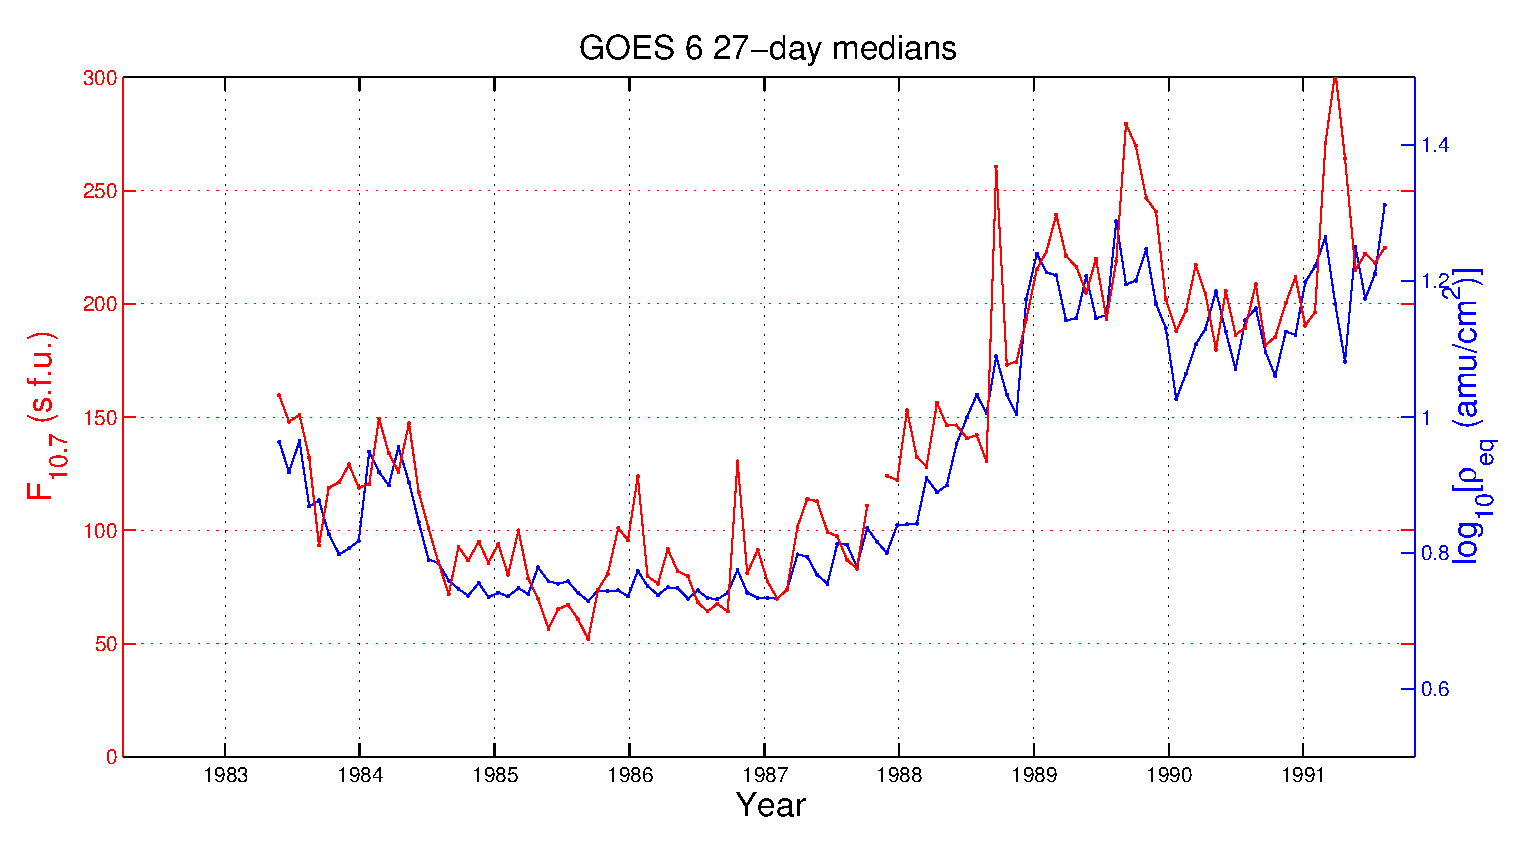
\includegraphics[scale=0.40]{figures/F107MD27d-GOES6.eps}
\includegraphics[scale=0.40]{figures/ccplot-GOES6.eps}
\caption{Top: 27-day non-overlapping medians of $F_{10.7}$ and $log(\rho_{eq})$ from GOES 6. Bottom: Correlation between $log(\rho_{eq})$ and $F_{10.7}$ using medians in non-overlapping hour, day, and 27-day windows.}
\label{ccplot}
\end{figure}
\clearpage

\begin{figure}[h]
\centering
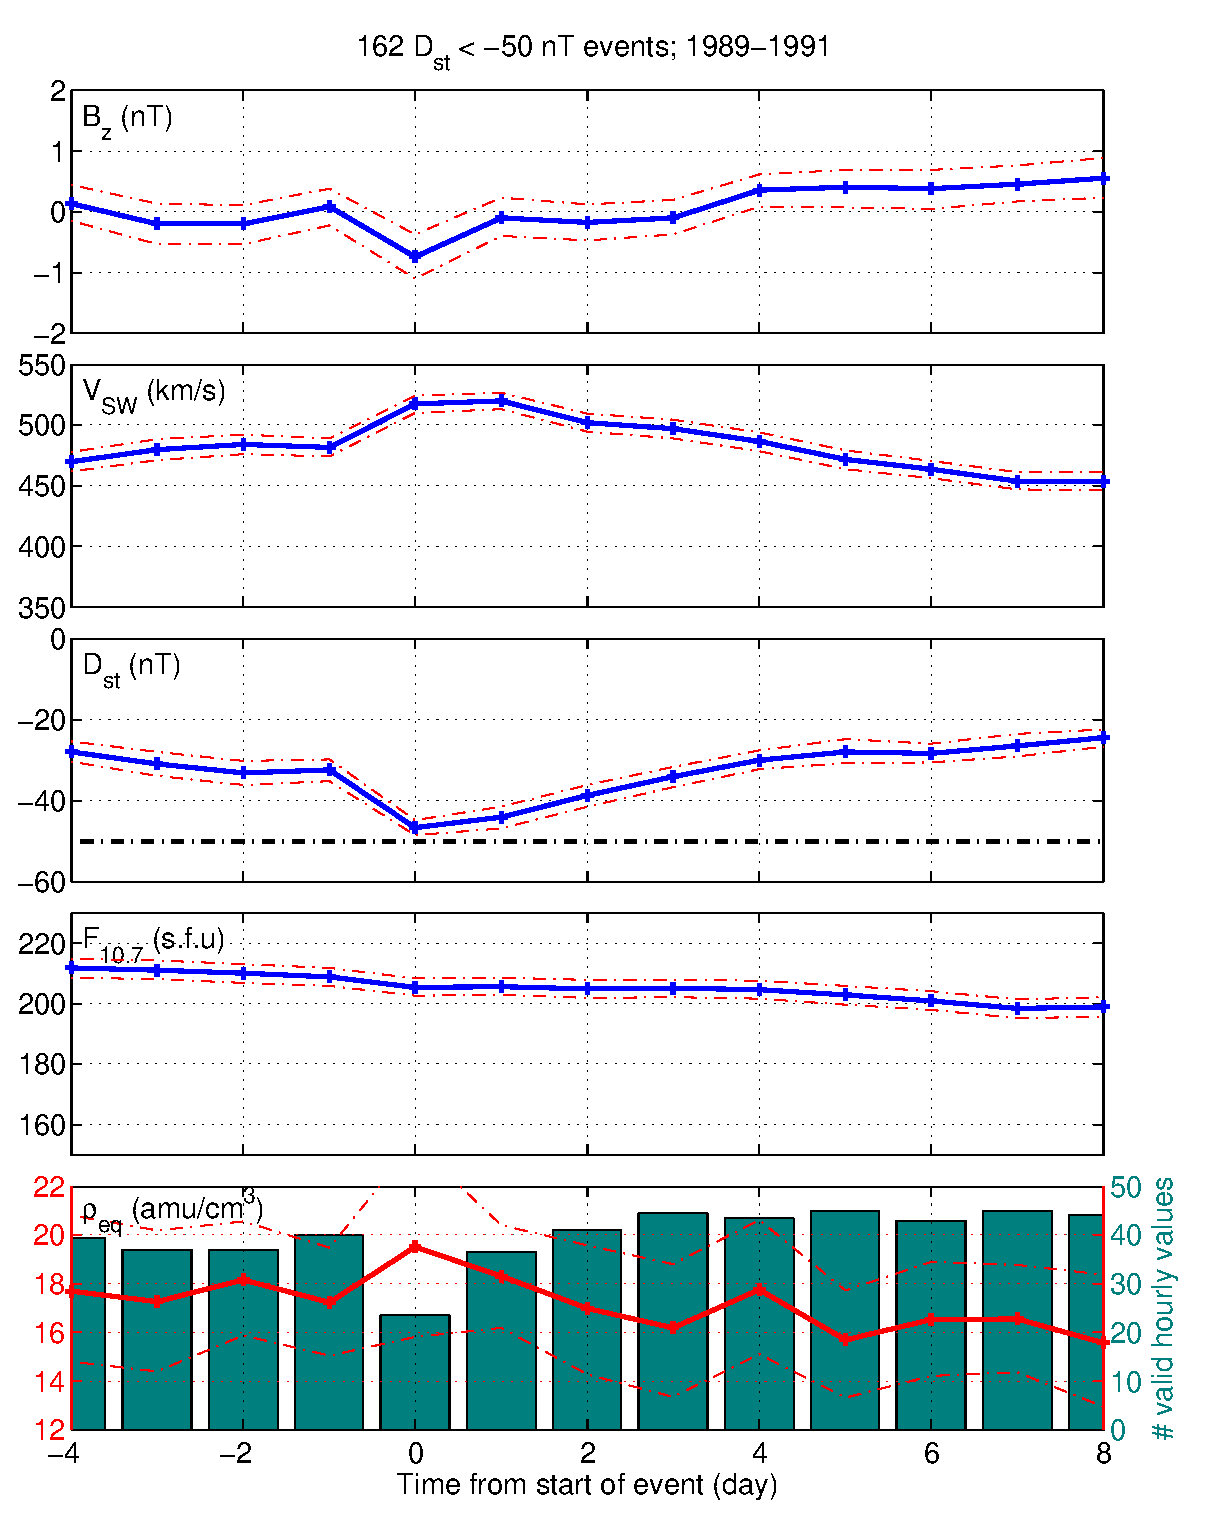
\includegraphics[scale=0.40]{figures/stormavs-dst-50-tak-GOES6.eps}
\\
\rule[1ex]{5cm}{1pt}
\\
\includegraphics[scale=0.40]{figures/stormavs-dst-day-GOES6.eps}
\caption{$D_{st}$ events from GOES 6 using daily medians. Top: Events in the interval 1989-1991; compare to \cite{Takahashi2010} Figure~11. Bottom: Events in the interval 1983-1991.}
\label{DailyAveragedDstEvents}
\end{figure}

\clearpage

\begin{figure}[tp!]
\centering
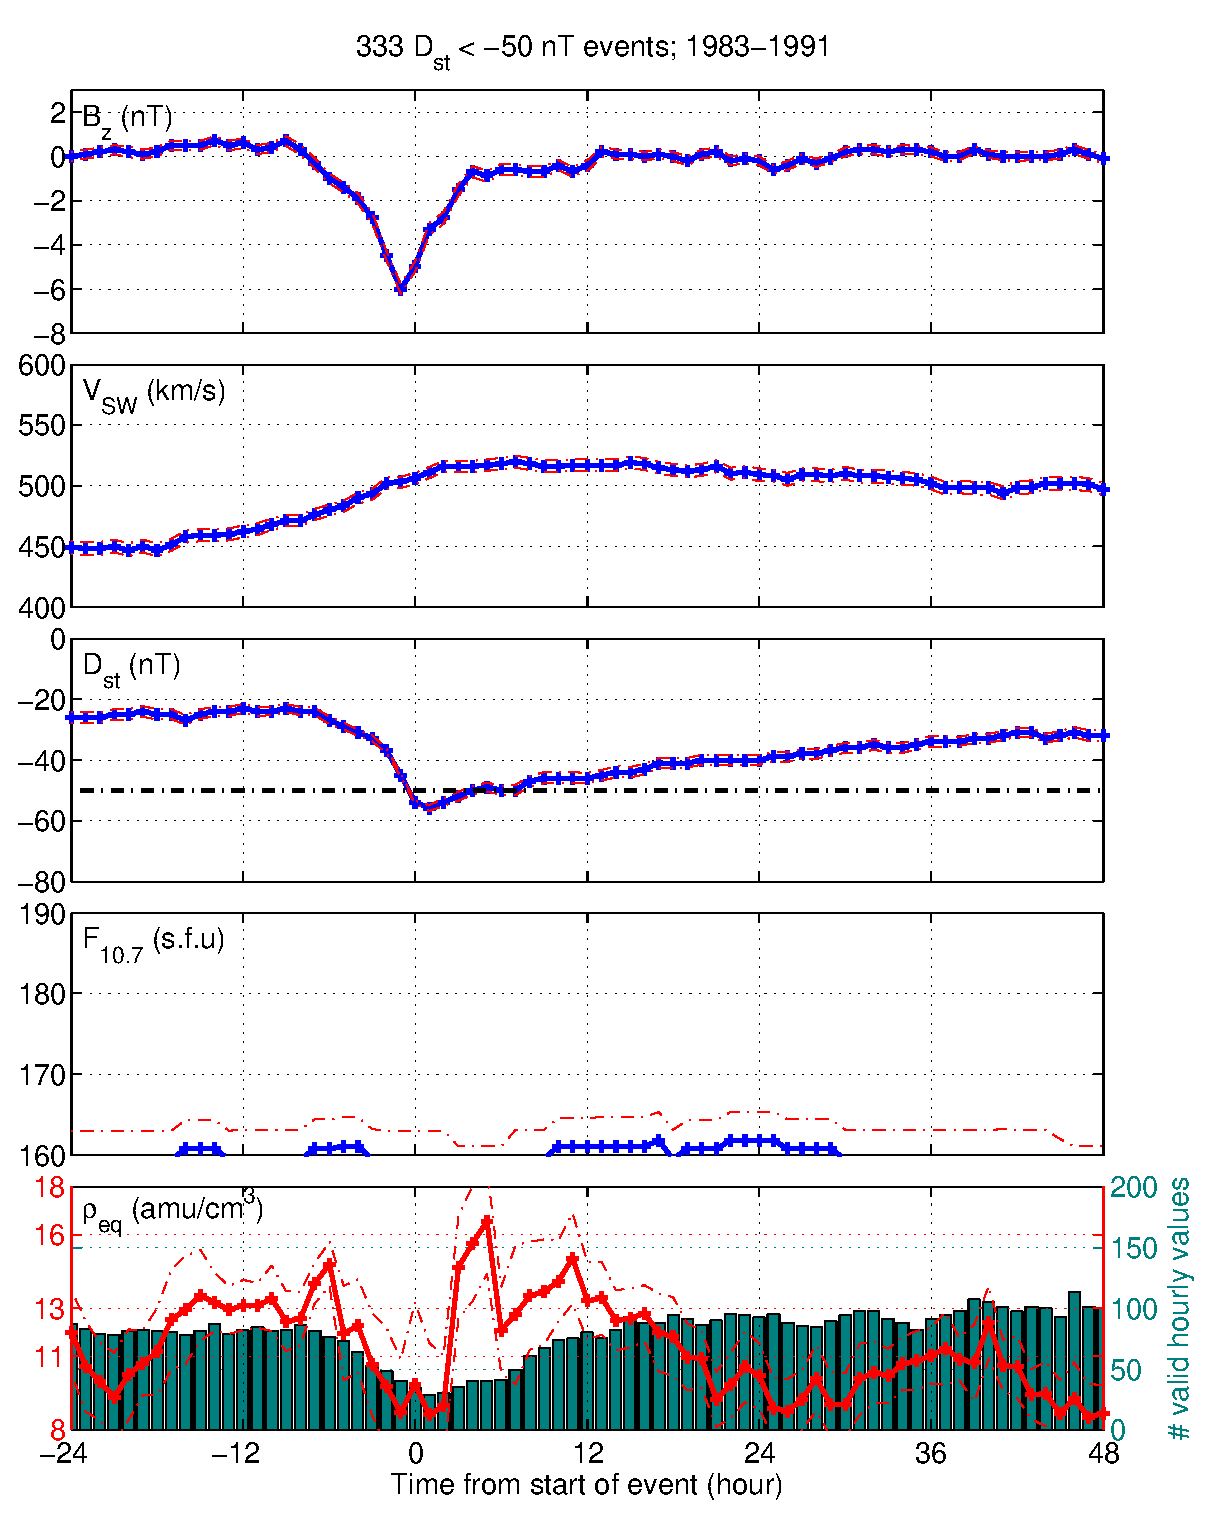
\includegraphics[scale=0.40]{figures/stormavs-dst-GOES6.eps}
\\
\rule[1ex]{5cm}{1pt}
\\
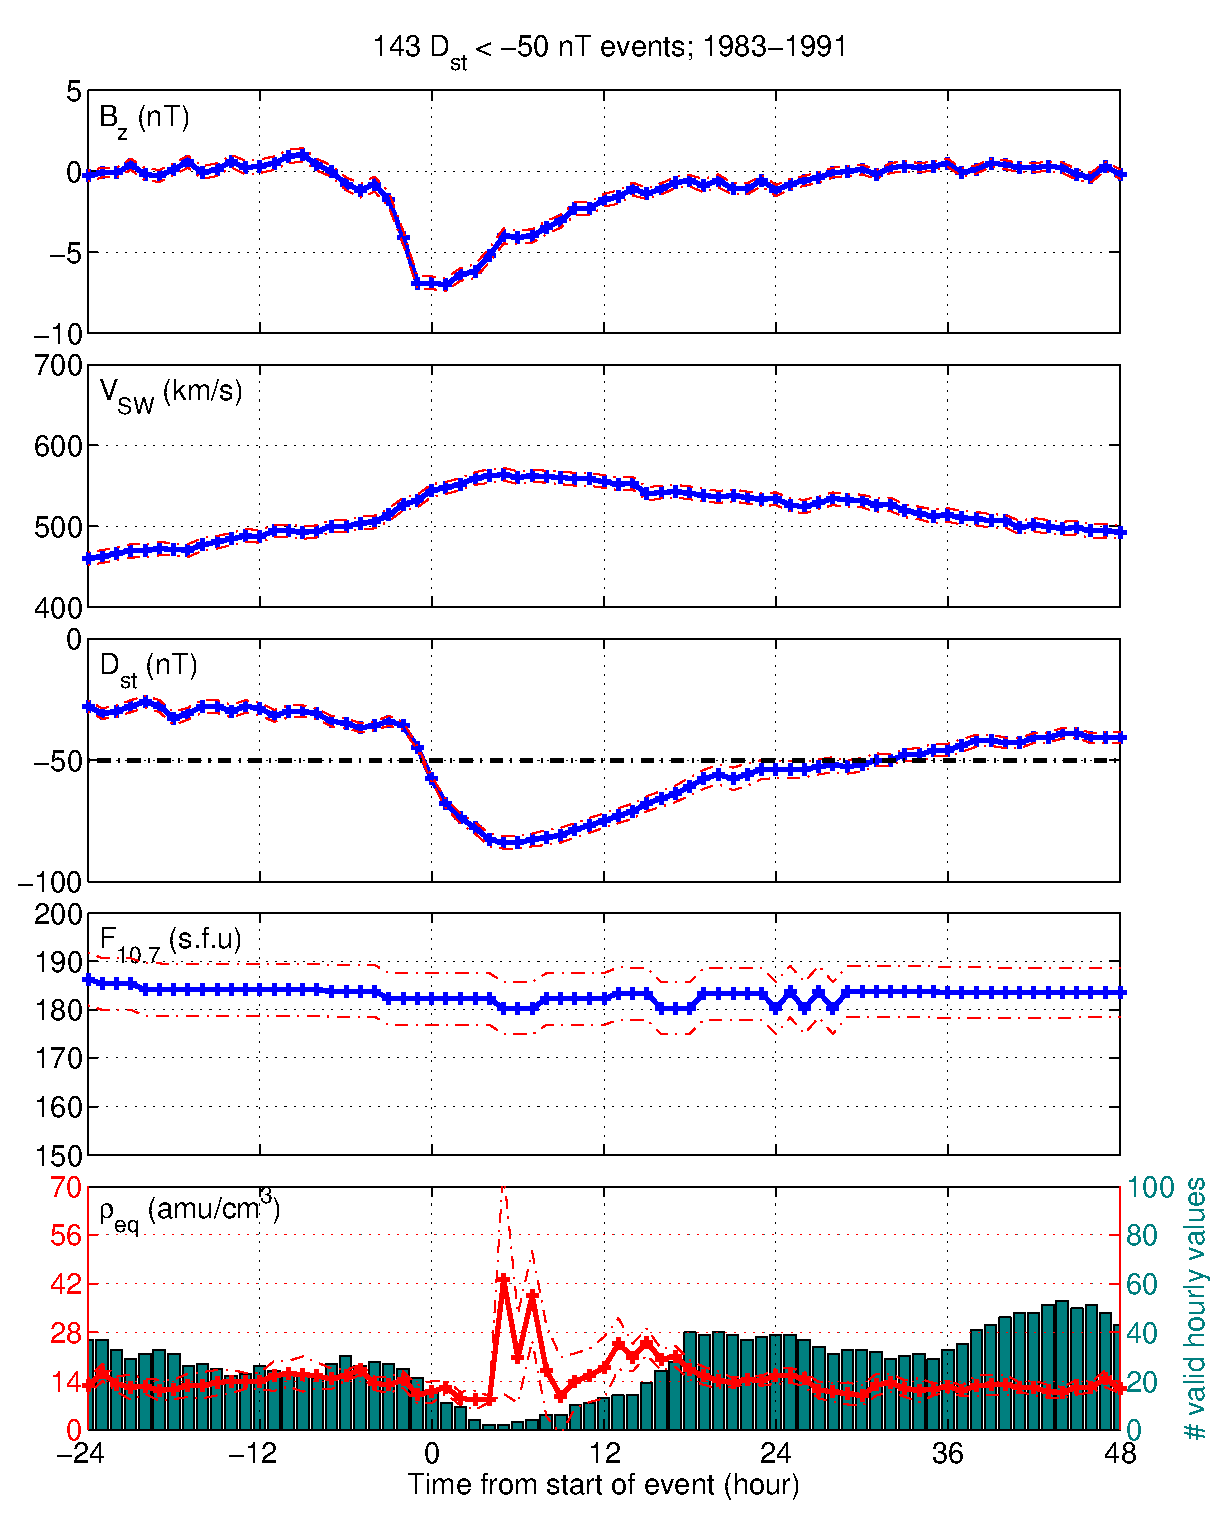
\includegraphics[scale=0.40]{figures/stormavs-dd12-GOES6.eps}
\caption{$D_{st}$ events from GOES 6 using hourly medians. Top: Events in the interval 1983-1991. Bottom: Same as Top except for constraint that $D_{st}$ stayed below $-50$~nT for at least 12~hours after crossing below $-50$~nT.}
\label{HourlyAveragedDstEvents}
\end{figure}

\clearpage
\begin{figure}[tp!]
  \centering
  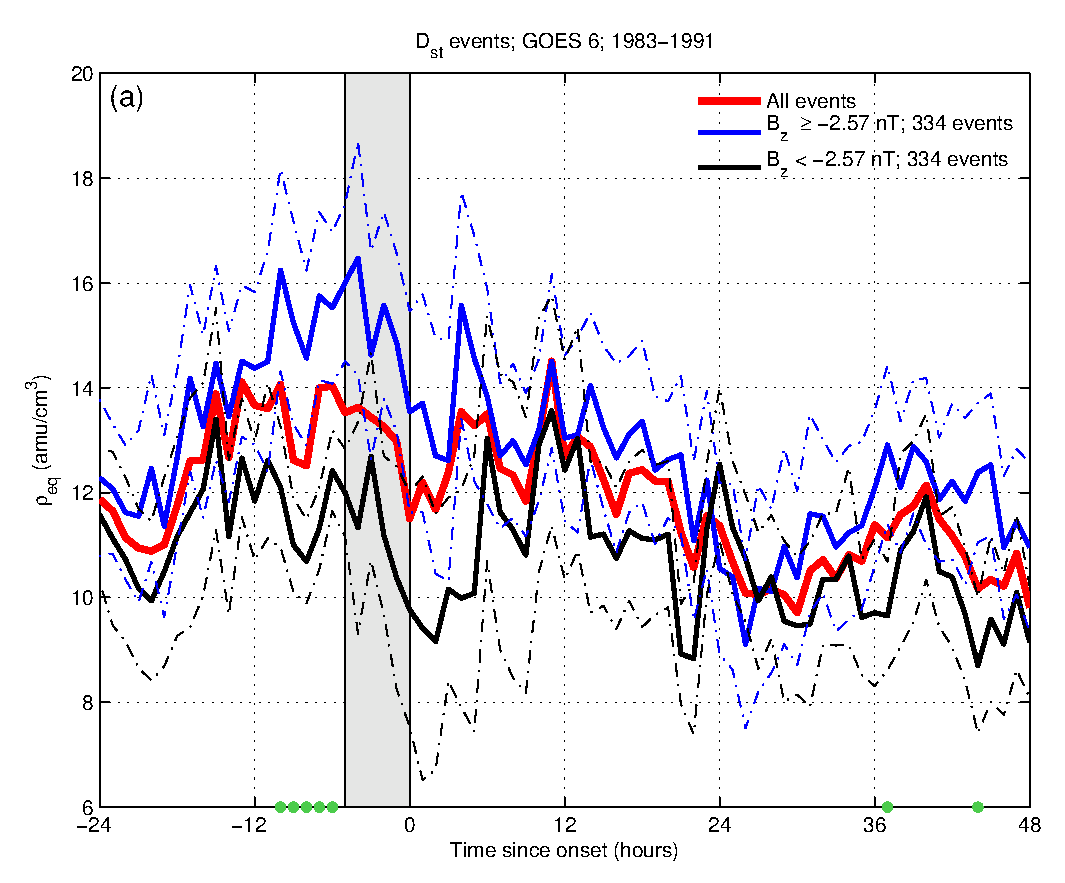
\includegraphics[scale=0.40]{figures/RhoBinned/RhoBinnedB_z-case1-t020-tf25-GOES6.eps}
  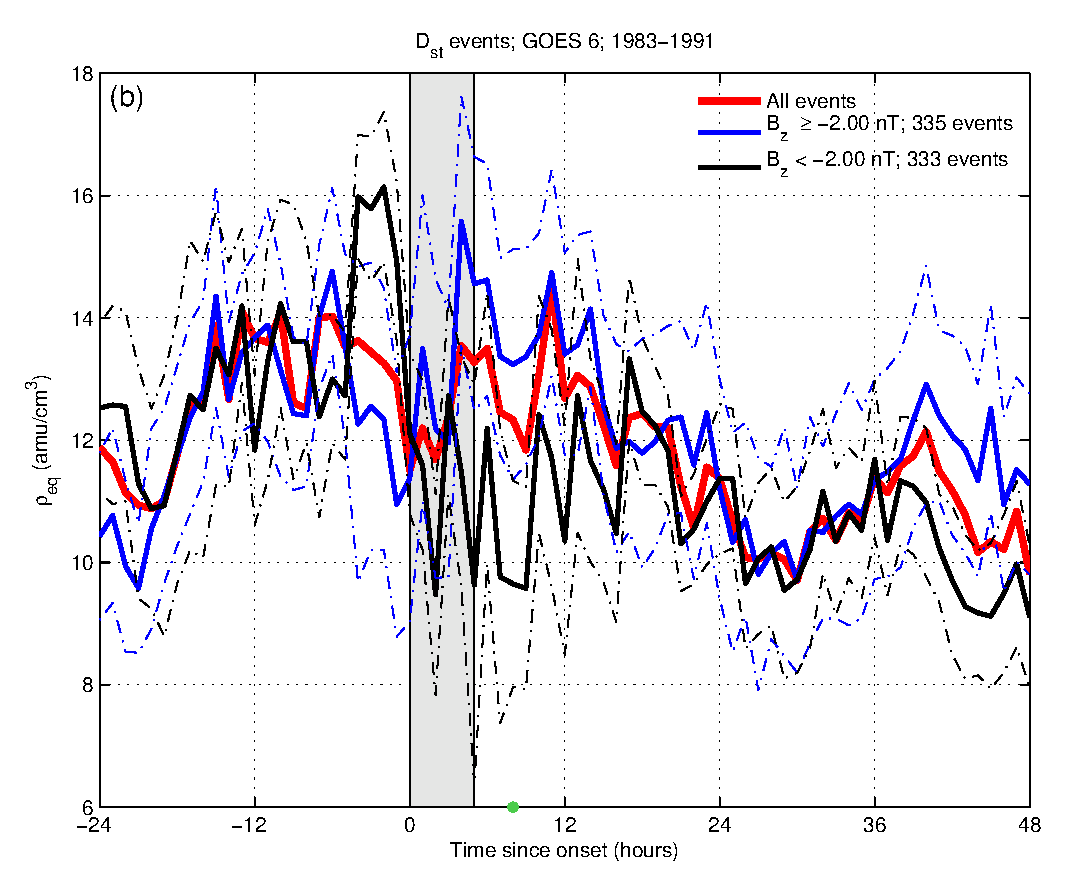
\includegraphics[scale=0.40]{figures/RhoBinned/RhoBinnedB_z-case1-t025-tf30-GOES6.eps}
  \caption{$D_{st}$ events of Figure~\ref{HourlyAveragedDstEvents} separated by the average $D_{st}$ value (a) at onset and four hours before, and (b) at onset and four hours after.}
  \label{fig:BzBinnedDstEvents}
\end{figure}

\begin{figure}[tp!]
  \centering
  \includegraphics[scale=0.40]{figures/RhoBinned/RhoBinnedF_{10.7}-case1-t020-tf25-GOES6.eps}
  \includegraphics[scale=0.40]{figures/RhoBinned/RhoBinnedF_{10.7}-case1-t025-tf30-GOES6.eps}
  \caption{$D_{st}$ events of Figure~\ref{HourlyAveragedDstEvents} separated by the average $F10.7$ value (a) at onset and four hours before, and (b) at onset and four hours after.}
  \label{fig:F107BinnedDstEvents}
\end{figure}

\clearpage

\begin{figure}[htp!]
\centering
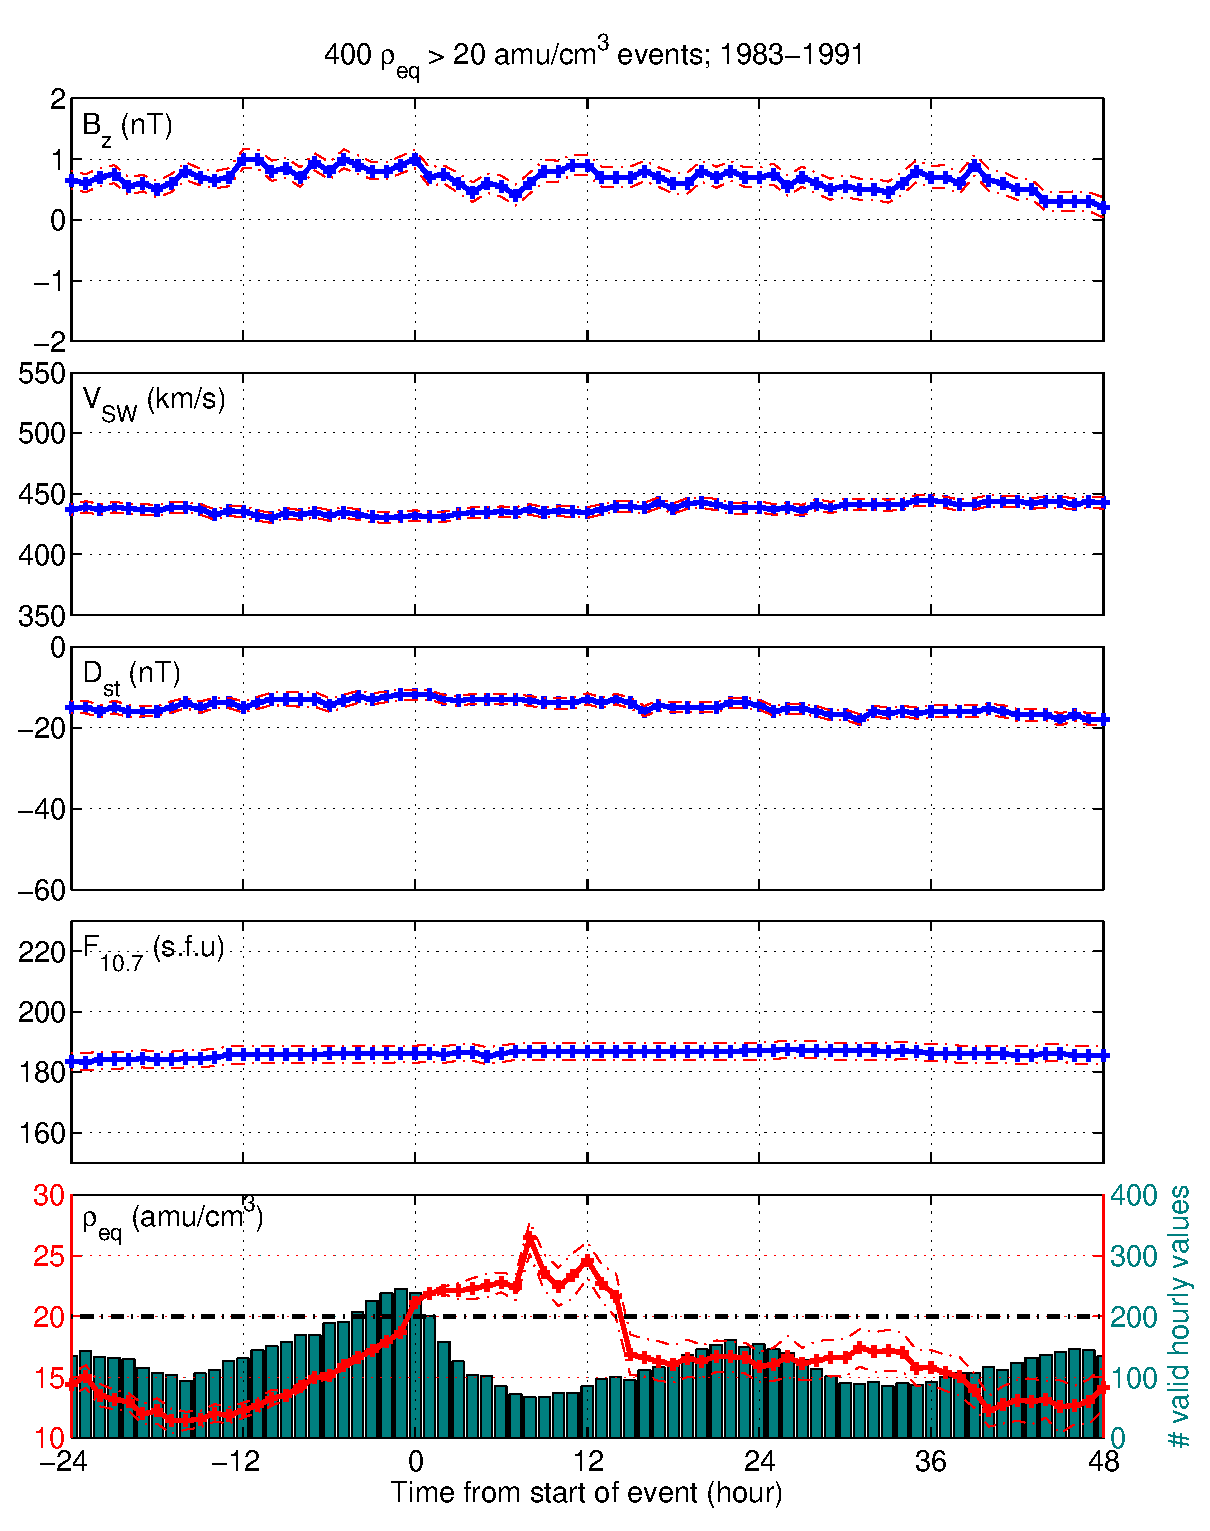
\includegraphics[scale=0.40]{figures/stormavs-mass-gt20-GOES6.eps}
\caption{$\rho_{eq} >$ 20~amu/cm$^3$ events from GOES 6 using hourly medians.}
\label{HourlyAveragedRhoEvents}
\end{figure}

\clearpage
\begin{figure}[tp!]
  \centering
  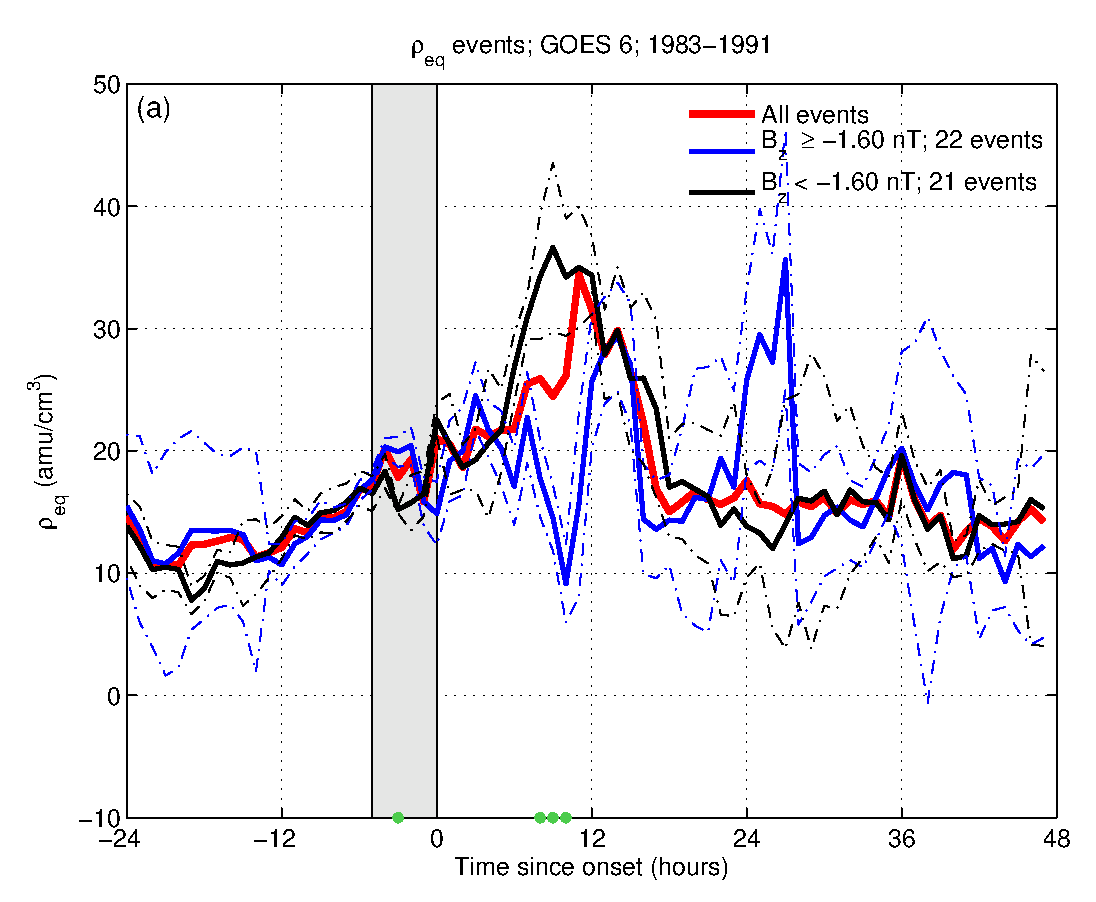
\includegraphics[scale=0.40]{figures/RhoBinned/RhoBinnedB_z-case24-t020-tf25-GOES6.eps}
  \includegraphics[scale=0.40]{figures/RhoBinned/RhoBinnedB_z-case24-t025-tf30-GOES6.eps}
  \caption{$\rho_{eq}$ events of Figure~\ref{HourlyAveragedRhoEvents} separated by the average $B_z$ value (a) at onset and four hours before, and (b) at onset and four hours after.}
  \label{fig:BzBinned}
\end{figure}

\begin{figure}[tp!]
  \centering
  \includegraphics[scale=0.40]{figures/RhoBinned/RhoBinnedF_{10.7}-case24-t020-tf25-GOES6.eps}
  \includegraphics[scale=0.40]{figures/RhoBinned/RhoBinnedF_{10.7}-case24-t025-tf30-GOES6.eps}
  \caption{$\rho_{eq}$ events of Figure~\ref{HourlyAveragedRhoEvents} separated by the average $F10.7$ value (a) at onset and four hours before, and (b) at onset and four hours after.}
  \label{fig:F107Binned}
\end{figure}

\end{document}
